\documentclass[11]{article}
\usepackage{amsmath}
\usepackage[inline]{enumitem}
\usepackage{graphicx}
\usepackage{gensymb}
\usepackage{float}
\newcommand{\dd}[1]{\mathrm{d}#1}
\usepackage{hyperref} 

\usepackage[T1]{fontenc}
\usepackage[utf8]{inputenc}
\usepackage[font=small,labelfont=bf]{caption}

\usepackage[dvipsnames]{xcolor}

\usepackage{bm}

\author{Adrian Ionita}

\title { Implementation Report for\\
Optimal Gaze Control\\
  \normalsize (multi-motor system) }

\begin{document}
\maketitle 	

\section{Introduction}
This document describes the implementation of optimal gaze control through reinforcement learning, as executed during the research placement. The code, sample results, and supporting documents can be found at \\
\href{url}{https://github.com/iceiony/gaze-control/}. 

Focus will be given to code inside the 'multi-motor' folder, which contains the final implementation. Background work supporting the project were Nunez-Valera's gaze control models\cite{nunezvalera} and Rashej Rao's decision making under uncertainty\cite{rashejrao}.

\section{Experimental Setup}
The experimental setup is similar to a visual perception task. Objects of different reward values are randomly placed on the screen. The objects are shown for a brief moment after which the subject must click on the locations where he thought the objects were located. 

Similarly, our learning agent is trained in a two dimensional environment (width 700px , height 500px). Two objects of different reward values are randomly placed on the screen (fig \ref{fig:scene}). The agent is allowed a single visual fixation after which it must decide to either \textit{grasp} or not to at the objects locations. If the agent misses the object center by more than 11px, a punishment is given. To motivate the agent to use both hands for grasping, a small punishment is given for not using one of the hands. Table \ref{table:rewards} shows the rewards and punishments for different agent actions.


  \begin{minipage}[b]{0.39\textwidth}
    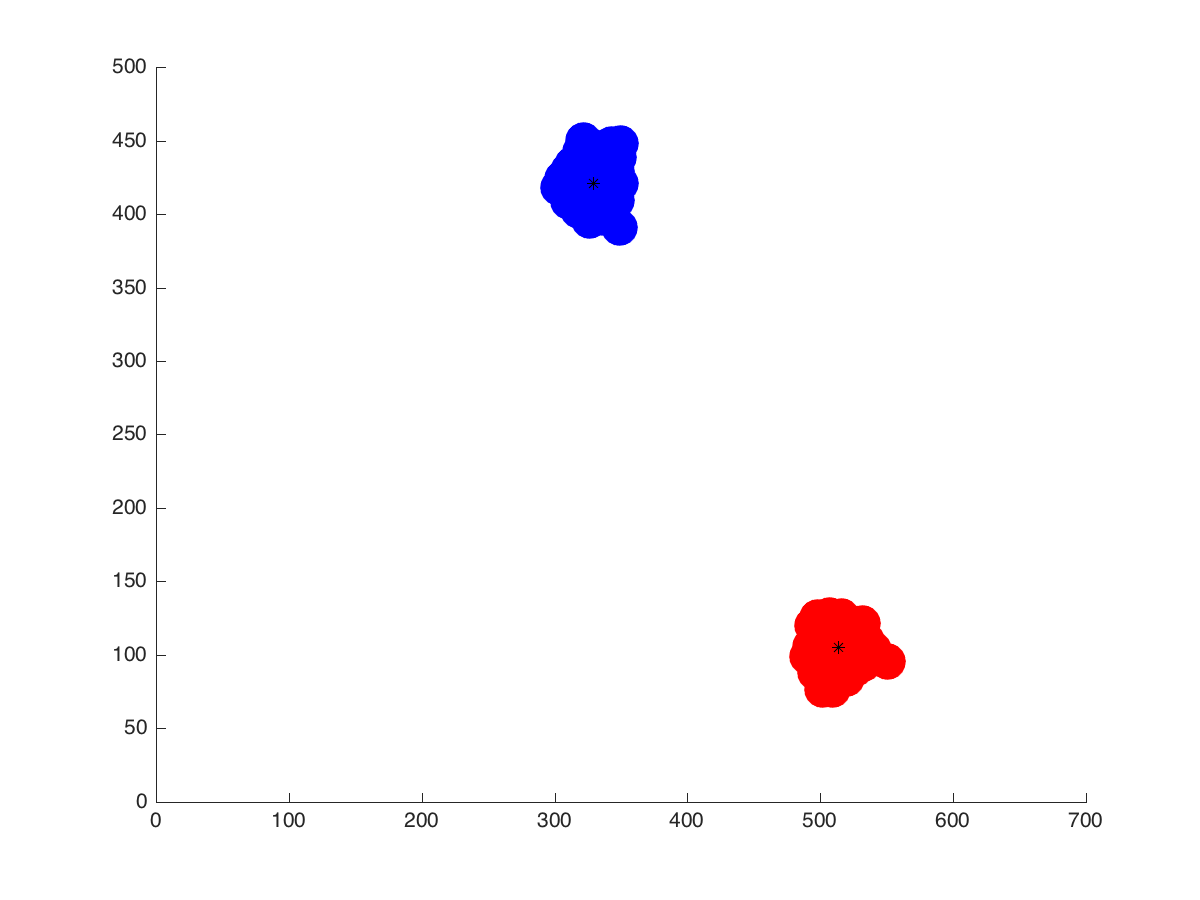
\includegraphics[width=1\textwidth]{Scene.png}
    \captionof{figure}{Scene}
    \label{fig:scene}
  \end{minipage}
  \hfill
  \begin{minipage}[b]{0.60\textwidth}
    \centering
    \begin{tabular}{cc}\hline
        \textbf{Reward} & \textbf{Action Condition}\\ \hline
        
        \textcolor{ForestGreen}{+30} & Grasp \textbf{\textcolor{red}{red}} object \\
        \textcolor{ForestGreen}{+10} & Grasp \textbf{\textcolor{blue}{blue}} object \\
        \textcolor{OrangeRed}{-100} & Miss object grasp by 11px \\
        \textcolor{OrangeRed}{-1} & Left hand not used \\
        \textcolor{OrangeRed}{-1} & Right hand not used \\ \hline
        \\
        
      \end{tabular}
      \captionof{table}{A table beside a figure}
      \label{table:rewards}
    \end{minipage}
 
The visual information received is perturbed by noise. As with human ocular fixations, the further the gaze center is from an object the more it's position is perturbed by noise. The amount of positional displacement added follows the function in figure \ref{fig:noise}. The distance to an object is normalised to the scene's dimensions. 

\begin{figure}[h]
	\centering
	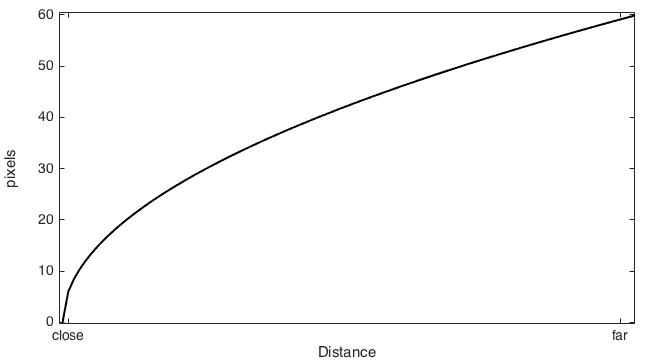
\includegraphics[width=0.7\textwidth]{Noise.png}
	\caption{Function of noisy displacement as distance increases}
	\label{fig:noise}
\end{figure}
 
\section{Representing Uncertainty}
It is assumed that the brain may rely on Bayesian inference in order to determine the true state of the world. As visual information is collected through ocular fixations our belief about the true state of the world becomes more and more precise. This process is especially important in the field of robotics, where sensory uncertainty has to be handled regardless of the quality of the hardware used.  

In our context we must handle the uncertainty of noisy visual information. This is done using particle filters for each individual object. Initially as no visual information exists  particles are spread across the entire scene(fig. \ref{fig:uncertainty} top). When new visual samples are received, the particles gather around the objects approximating their location more accurately with each successive input(fig. \ref{fig:uncertainty} bottom two). The spread of particles are therefore analogous to the representation of uncertainty. We denote them as the agent's belief state. 

\begin{figure}[h]
	\centering
	\includegraphics[width=0.7\textwidth]{uncertainty.png}
	\caption{Visual information decreasing uncertainty}
	\label{fig:uncertainty}
\end{figure}

\section{Learning}
The learning strategy used follows the methods described in Rashej Rao's approach \cite{rashejrao}. Our agent is trained over 8000 trials using reinforcement learning and an actor critic model(fig. \ref{fig:actor-critic}). 
\begin{figure}[h]
	\centering
	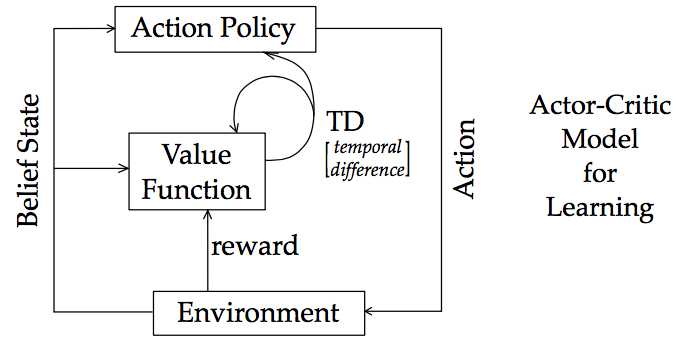
\includegraphics[width=0.7\textwidth]{actorcritic.png}
	\caption{}
	\label{fig:actor-critic}
\end{figure} 

The value function returns an expected reward for our current belief state. For example, in complete uncertainty the expected reward is low regardless of what action is taken. The difference over time steps in the value function's output is used for training an action policy. The action policy then returns the probability of taking an action given our current belief state.

There are two activities the agent has to learn: grasping and gazing. The actions are executed at the center of an object's particle spread and depend on the level of uncertainty. 

Both value function and action policy are learned using radial basis function(RBF) networks (fig. \ref{fig:rbf}).

\begin{figure}[h]
	\centering
	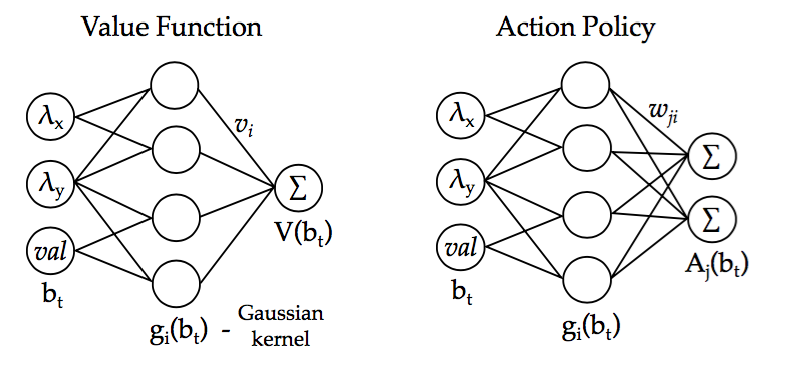
\includegraphics[width=0.7\textwidth]{rbf.png}
	\caption{}
	\label{fig:rbf}
\end{figure} 

\begin{list}{}{}
 \item $\pmb{b_t}$ - is the belief state. It is represented by the particle spread's eigen values and the object value (all normalised).
 \item $\pmb{g_i}$ - is a non-linear Gaussian kernel function ($\sigma=0.25$).  The kernel centers($\mu$), also known as belief points, are spread across a randomly generated range belief state values by k-means clustering. One third of the centers are randomly spread across the belief space.
Grasping has 60 kernel centers whilst gazing has 180.
 \item $\pmb{v_i}$ \& $\pmb{w_i}$ - output layer weights similar to a feed forward network
 \item $\pmb{V(b_t)}= \Sigma[v_i * g_i(b_t)]$ - value function
 \item $\pmb{A_j(b_t)}= \Sigma[w_{ji} * g_i(b_t)]$ - action value. Although network output is determined as $P_{action} = softmax(A_1(b_t),A_2(b_t))$; a normalised exponential
\end{list}

Grasp learning requires only a single object's uncertainty and value, whilst gazing  requires both. Figure \ref{fig:inout} is a graphical representation of input and output for both action policies.

\begin{figure}[h]
	\centering
	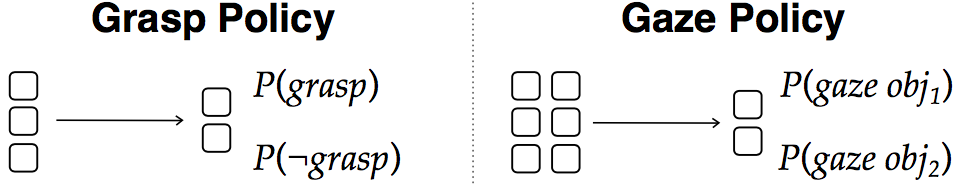
\includegraphics[width=0.7\textwidth]{inputoutput.png}
	\caption{}
	\label{fig:inout}
\end{figure}

\subsection{Grasp Learning}
When grasping, the action policy is simply a decision of executing a grasp or not. The decision is learned from the reward generated by the environment and follows these formulas : 
\begin{list}{}{}
  \item \textbf{reward =  from environment}; see table \ref{table:rewards}
  \item $\pmb{TD = reward + V(b_{t+1}) - V(b_t)}$; temporal difference
  \item $\pmb{ v_i = v_i + 0.001 * TD * g_i(b_t)}$; value function weights
  \item $\pmb{w_{ji} = w_{ji}+ 0.0005 * TD * g_i(b_t)}$; action policy weights
\end{list}  

\subsection{Gaze Learning}
In gaze learning, the action policy determines the probability of gazing at one of the objects. For optimal gaze we assume that gaze reward should be the sum of expected improvement over grasping reward. Grasping rewards correspond to probabilities, i.e. the probability of grasping grows as the value of grasping increases). Instead of using actual rewards we can therefore use the output of the grasping policy for gaze training.  : 
\begin{list}{}{}
  \item $\pmb{reward = \sum_{obj}[P_{grasp}(b_{t+1}) -  P_{grasp}(b_t)] }$; 
  \item $\pmb{TD = reward - V(b_t)}$; temporal difference
  \item $\pmb{ v_i = v_i + 0.8 * TD * g_i(b_t)}$; value function weights
  \item $\pmb{w_{ji} = w_{ji}+ 0.4 * TD * g_i(b_t)}$; action policy weights
\end{list}  

For either grasp or gaze learning, the belief points of each network could also have been moved similar to Rashej's technique \cite{rashejrao}. The approach was tested but did not render noticeable improvements. Learning success depends highly on the distribution of belief points. Future work should consider alternative strategies for this distribution. For example, considering k-means clustering over possible values of the belief space, as opposed to randomly generated values.

\pagebreak

\section{Results}
Both grasping and gazing were successfully learned. In order to establish a baseline for performance, reward was recorded from grasping whilst randomly gazing. 
Figure \ref{fig:results} shows the success of the learning technique and a large difference between an optimal gaze strategy vs random gazing. The graph is the result of learning using all the parameters previously described. The faded blue and red areas represent the standard error over 100 training runs.

\begin{figure}[h]
	\centering
	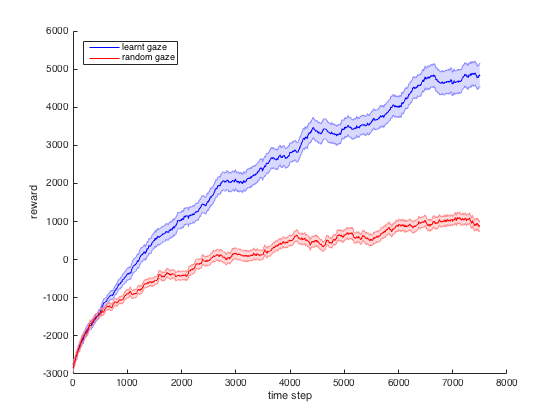
\includegraphics[width=0.7\textwidth]{results.png}
	\caption{}
	\label{fig:results}
\end{figure}

\subsection{Additional Results}
We also explored a scenario where the agent is allowed as many visual fixations as required before having to make grasp decisions. The agent is yet again allowed to grasp either object or both, although he may do so after becoming completely certain about the objects positions.

Figure \ref{fig:resultsTimless} shows that optimal gaze has a very small impact on overall task performance. However, when looking on the number of fixations, optimal gaze tends to fixate noticeably fewer times than random gaze (fig. \ref{fig:gazeCount}). Both figures contain the average and standard error collected over 20 training runs whilst using a 500 value moving window sum.

\begin{figure}[h]
	\centering
	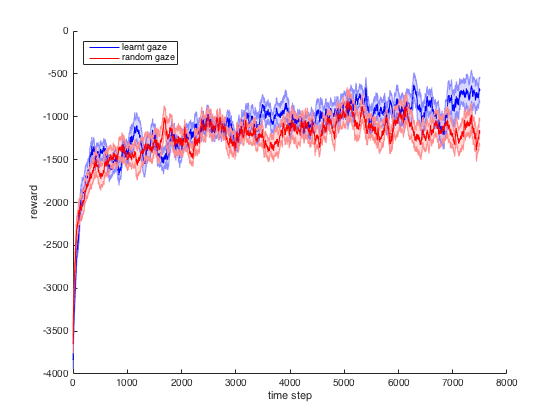
\includegraphics[width=0.7\textwidth]{resultsTimeless.png}
	\caption{Task performance for as many fixations as needed}
	\label{fig:resultsTimless}
\end{figure}


\begin{figure}[!h]
	\centering
	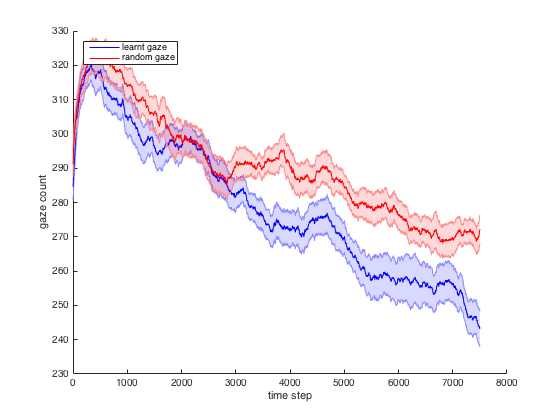
\includegraphics[width=0.7\textwidth]{gazeCount.png}
	\caption{Number of fixations before grasp (moving window sum)}
	\label{fig:gazeCount}
\end{figure}

\pagebreak

\begin{thebibliography}{9}
\bibitem{nunezvalera}
Nunez-Varela, J. and Wyatt, J. L. (2013) ‘Models of gaze control for manipulation tasks’, ACM Transactions on Applied Perception, 10(4), pp. 1-22. doi: 10.1145/2536764.2536767.

\bibitem{rashejrao}
Rao, R. P. N. (2010). Decision making under uncertainty: A neural model based on partially observable Markov decision processes. Frontiers in Computational Neuroscience, 4, . doi:10.3389/fncom.2010.00146

\end{thebibliography}

\end{document}